\chapter{Design of circuit}
  
  \section{DC Bias point at gate}

  We are using ADS to simulate the I-V characteristics of the CGH40010 transistor. ADS is providing a built-in design guide for this purpose. Figure~\ref{fig:fig_IV} shows the I-V characteristics, with drain current on the y-axis, drain voltage on the x-axis and curves for various gate voltages from -5 to -1 volts in 0.2 volts increments. Refering to figure 5.12 in \cite[p.~200]{AmpRobertson}, we choose to set a bias point at approximately 70\% of the maximum saturated drain current IDS, to achieve a compromise between good linearity and high gain. We find this to be a gate voltage of about -1 volts.

  \begin{figure}[h]
	  \label{fig:fig_IV}
	  \centering
	  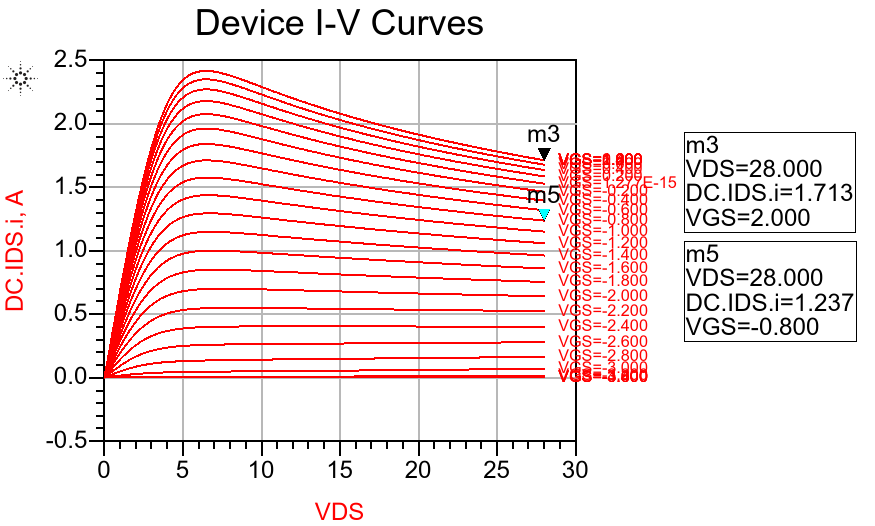
\includegraphics[width=0.75\textwidth]{img/01_IVCurve.png}
	  \caption{I-V curve characteristics for CGH40010}
  \end{figure}

  \section{Stability}

  \subsection{Calculations}
  Table~\ref{tab:cree_sparm} lists the S-Parameters for the transistor as given in \cite{CreeDS}. Using these, we can calculate the $K$ and $\lvert \Delta \rvert$ factors to determine the stability using equations (6.31) and (6.32) in \cite{Pozar}.
  \begin{table}[h]
	  \label{tab:cree_sparm}
	  \centering
  \begin{tabular}{l l}
	  $S_1$$_1$ & $0.9 \angle 165^{\circ}$ \\
	  $S_{12}$ & $0.019 \angle -17.6^{\circ}$ \\
	  $S_{21}$ & $4.21 \angle 46.9^{\circ}$ \\
	  $S_{22}$ & $0.39 \angle -162^{\circ}$ \\
  \end{tabular}
  \caption{S-parameters for Cree CGH40010}
  \end{table}

  Using these values we find $K = 0.732$ and $\lvert \Delta \rvert = 0.282$. \emph{Rollet's condition} specifies that an amplifier will be unconditionally stable if $K > 1$ and $\lvert \Delta \rvert < 1$. Since only the latter condition is fulfilled in our case, the transistor will not be unconditionally stable by itself.


  \section{Gate bias network}
  The purpose of a bias network is to filter unwanted noise from the bias voltage source to prevent it from reaching the gate, and to prevent RF signal from the amplifier input from reaching the bias voltage source. Our gate bias network is composed of a microstrip quarter-wave transformer which blocks the input signal from reaching the bias source, and a capacitor bank that filters out noise from the bias voltage source.

  Figure~\ref{fig:Biasschem} shows the bias network we are using, with the probes used for measuring S-parameter characteristics. We have first simulated the two-port characteristics with terminal 1 at the input and terminal 2 at the point that will be connected to the transistor's gate. Figure~\ref{fig:Biastwos} shows two-port parameters $S_1$$_2$ and $S_2$$_2$, which shows that within our designated frequency band from 2.35 to 2.45 GHz, only between -42 and -50 dB of the input signal gets transmitted to the bias voltage source.

  We have also simulated one-port S-parameters by grounding the input of the circuit and measuring the reflection coefficient at the output ($S_1$$_1$). This is more relevant to real-world conditions as the DC voltage source providing the bias voltage will act as an AC ground. The results of this simulation is shown in figure~\ref{fig:Biasones}. The simulation shows that within the 2.35-2.45 GHz band almost all of the incident wave is reflected, while we have a -6dB attenuation of the reflected incident wave at approx. 1.8 GHz.

  \begin{figure}[h]
	  \label{fig:Biasschem}
	  \centering
	  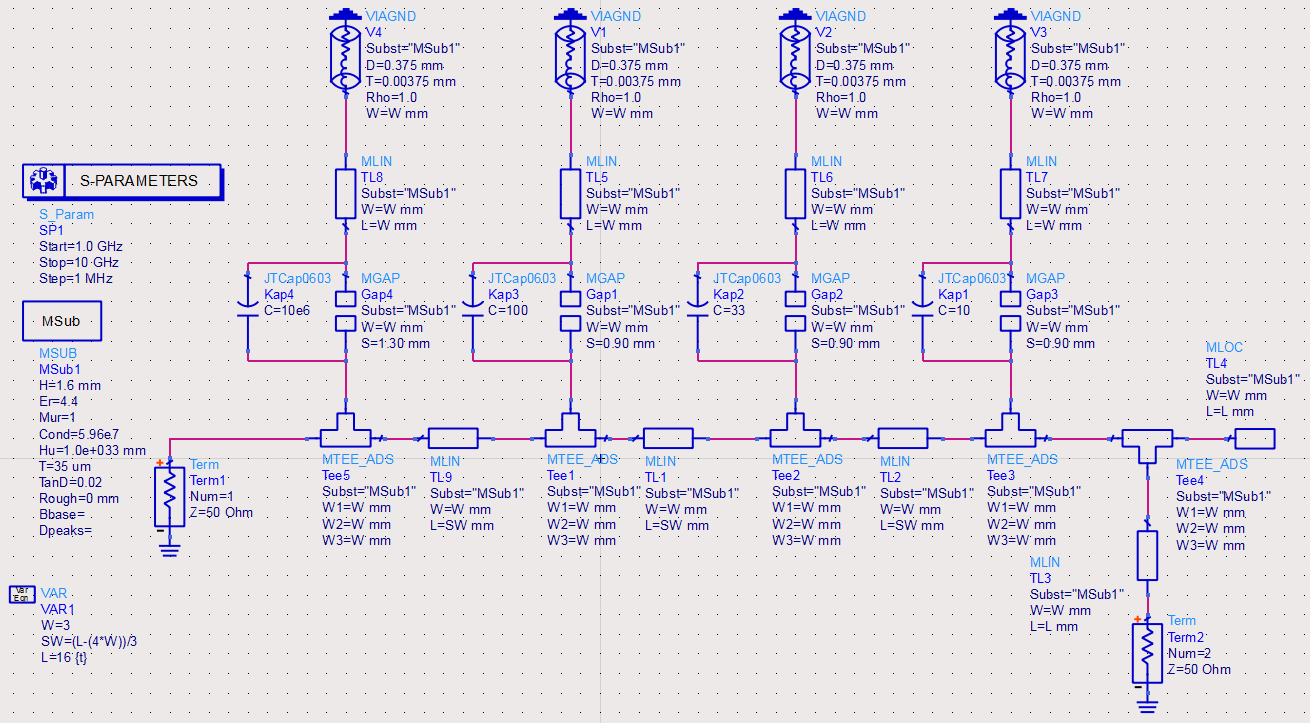
\includegraphics[width=\textwidth]{img/Bias_filter_two_port}
	  \caption{Gate bias network schematics}
  \end{figure}

  \begin{figure}[h]
	  \label{fig:Biastwos}
	  \centering
	  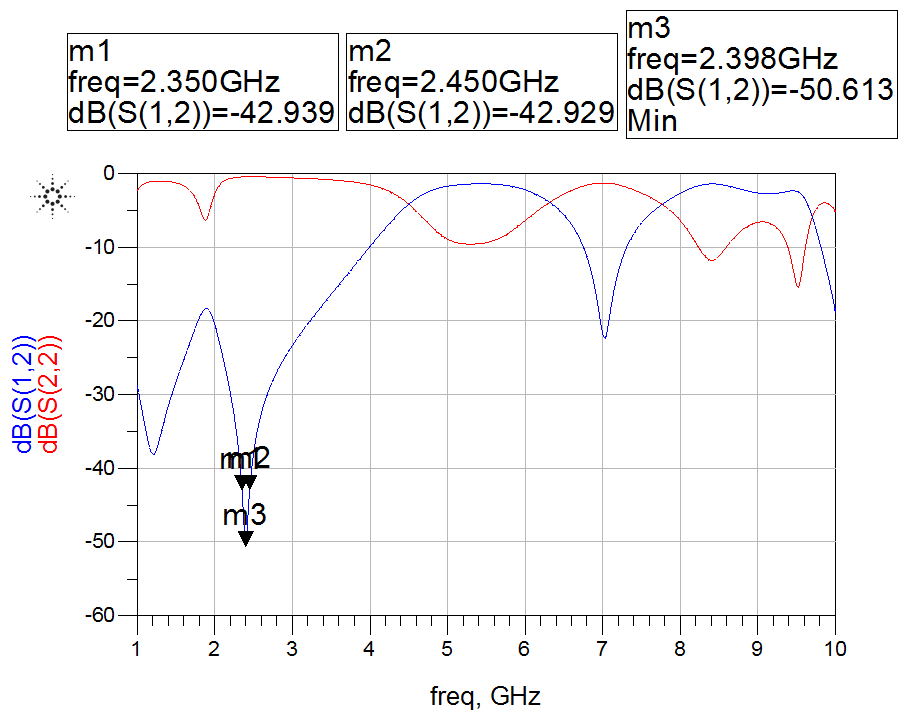
\includegraphics[width=0.75\textwidth]{img/Bias_filter_two_port_s_parm}
	  \caption{Bias network two-port S-parameter}
  \end{figure}

  \begin{figure}[h]
	  \label{fig:Biasones}
	  \centering
	  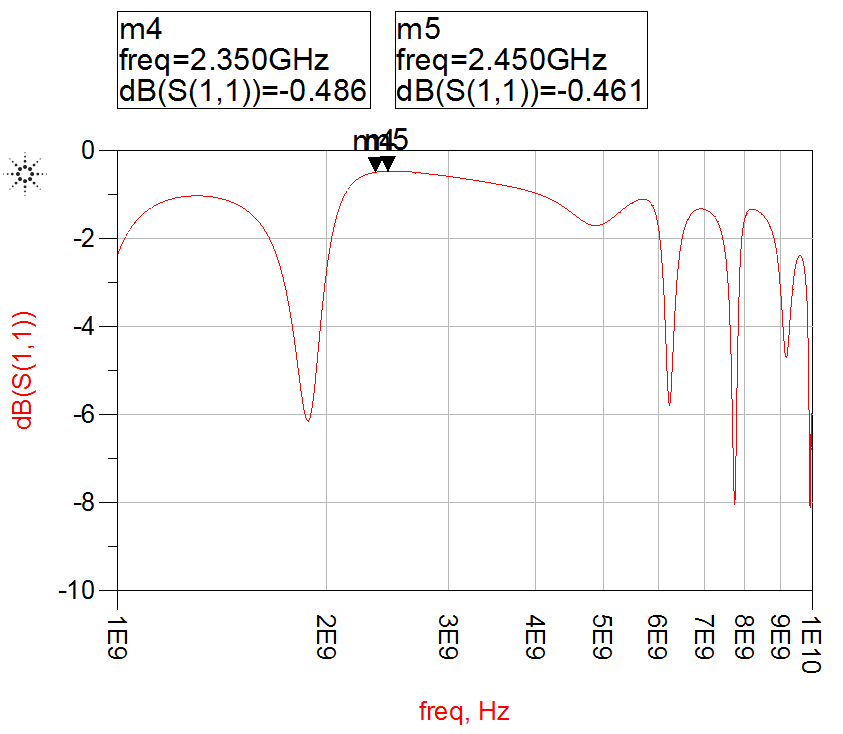
\includegraphics[width=0.75\textwidth]{img/Bias_filter_one_port_s_parm}
	  \caption{Bias network one-port S-parameter}
  \end{figure}

  \section{Matching network}
